\section{Quasi Experiment EE13.1}




%%
\begin{frame}[fragile]{EE12.2}

我們直接從課本的Empirical Exercise 13.1來複習如何用Stata實作quasi-experimental analysis,並做出解釋。

\end{frame}

%%
\begin{frame}[fragile]{EE13.1 Questions}
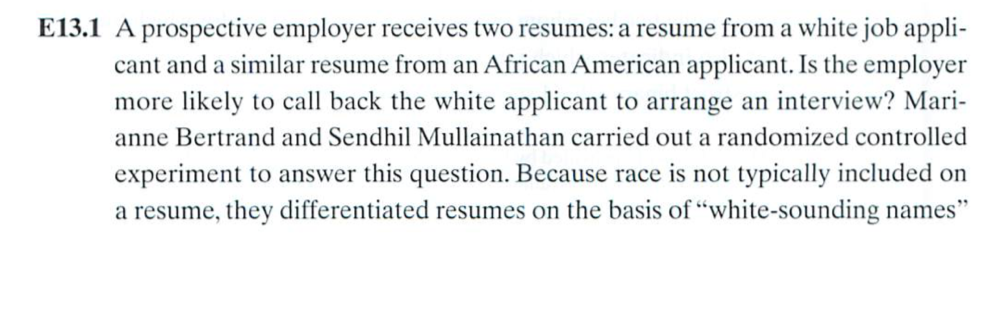
\includegraphics[width=1\textwidth]{Images/EE13-1_1.png}
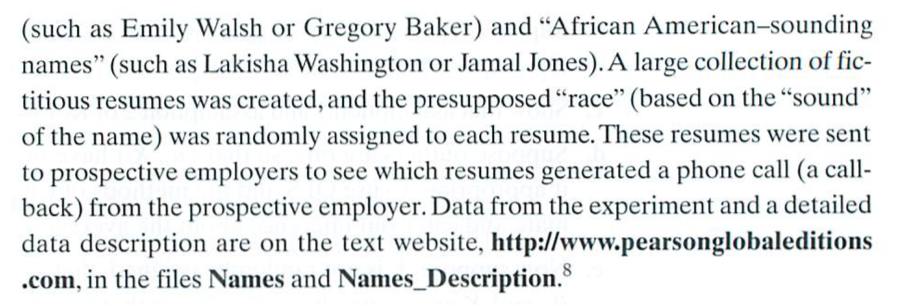
\includegraphics[width=1\textwidth]{Images/EE13-1_2.png}
\end{frame}
%%
\begin{frame}[fragile]{EE13.1 Questions}
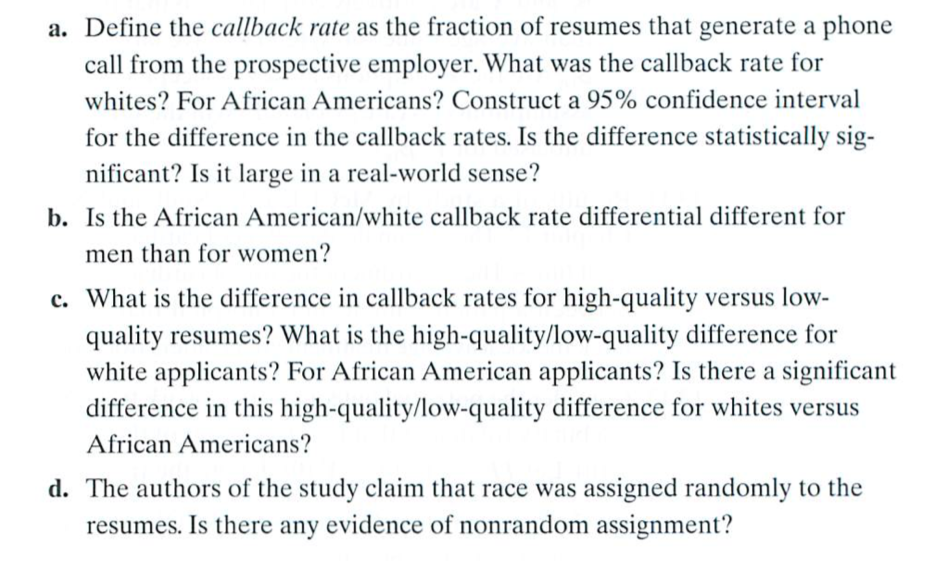
\includegraphics[width=1\textwidth]{Images/EE13-1_3.png}
\end{frame}



%%
\begin{frame}[fragile]{EE13.1 Data Descrptions}

Names Data

\begin{enumerate}
    \item Observations: 4870 resumes
    \item Time Period : 2001
\end{enumerate}
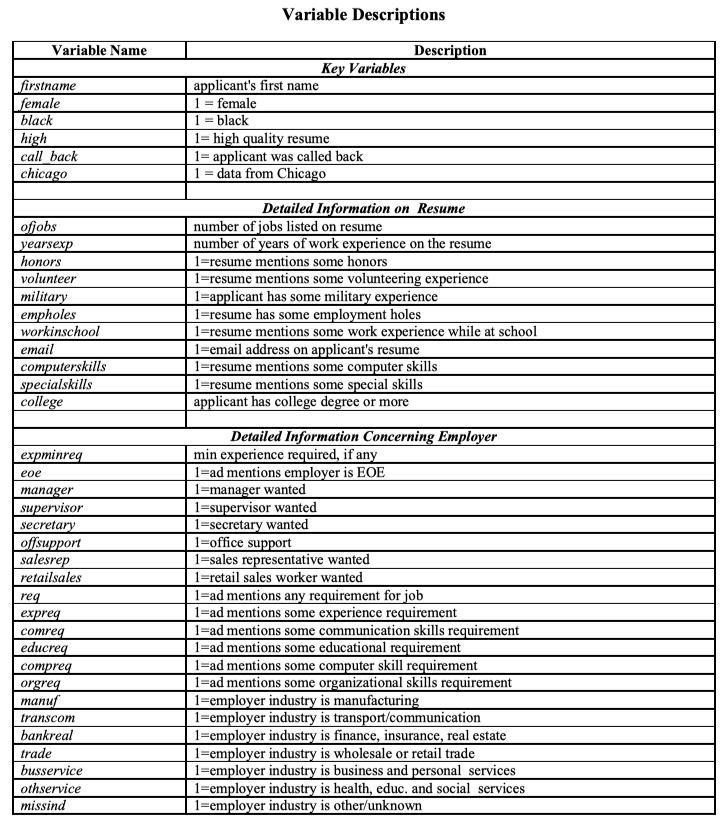
\includegraphics[width=0.5\textwidth]{Images/EE13-1_4.png}

\end{frame}


%%
\begin{frame}[fragile]{EE13.1 a}

The command:

\texttt{mean callback} 

gives us the fraction of resumes that generate a phone call from prospective employer.

The expression:

\texttt{ci mean callback} 

gives us the same result.
\end{frame}


%%
\begin{frame}[fragile]{EE13.1 a}

For whites, simply add a condition:

\texttt{ci mean callback if black==0}

For blacks:

\texttt{ci mean callback if black==1}

\end{frame}


%大刮號binary寫法:https://blog.csdn.net/miao0967020148/article/details/78712811
%
\begin{frame}[fragile]{EE13.1 a conti.}

To understand how Stata gives us the 95\% C.I., recall the point estimator in the previous semester.

Let $$ y_i=\left\{
\begin{aligned}
1 & , \text{if receive phone call}\\
0 & , \text{o.w.}\\
\end{aligned}
\right.$$

Clearly, $y_i$ follows $Bernoulli(p)$ where $p$ is the unknown fraction of resumes that generate a phone call from prospective employer.

Naturally, we would like to use $\bar{y} = \frac{1}{n}\sum_{i=1}^n y_i$ to estimate $p$. Where $n=4870$.

We need to know $se(\bar{y})$ in order to build up a interval estimator.

\end{frame}


%
\begin{frame}[fragile]{EE13.1 a conti.}

Now, our concern would be: What is the sampling distribution of $\bar{y}$?

Given $$y_i \stackrel{i.i.d.}{\sim} Bernoulli(p)$$

then $$\sum_{i=1}^n y_i \sim Binomial(n, p)$$

which can be approximated by normal distribution $$\sum_{i=1}^n y_i \stackrel{a}{\sim} N(np, np(1-p))$$ as $n \rightarrow \infty$. And let $X = \frac{1}{n} \sum_{i=1}^n y_i$, then $$X \sim N(p, \frac{p(1-p)}{n})$$

That is, $se(\bar{y})$ can be calculated easily from the approximated normal distribution.
\end{frame}


%
\begin{frame}[fragile]{EE13.1 a conti.}

With the normal quantile $Z_{0.05} = -1.96$, we know the interval estimator for $p$ is:


[$ \bar{y}-1.96\times se(\bar{y}), \bar{y}+1.96 \times se(\bar{y}) $]


And we know $se(\bar{y}) \approx (0.0804928(1-.0804928)/4870)^{\frac{1}{2}} = 0.003898446728$

Which is nearly the \texttt{Std. Err.} calculated by Stata.

After that, we may construct the C.I. under every given quantile.

\end{frame}


%
\begin{frame}[fragile]{EE13.1 a conti.}

Some may know that the command:

\texttt{ci proportion callback}

gives us a very similar result, and wonder the difference between the two.

Actually, you may see the text "Binomial Exact" in the latter command.

That is, Stata calculate the exact sampling distribution from "categories" we're interested in, instead of using the approximated normal distribution.

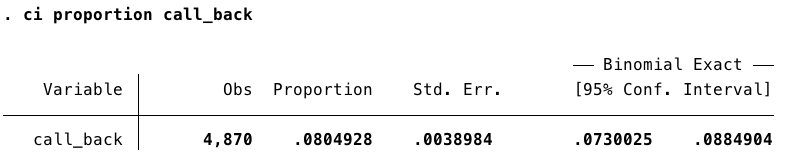
\includegraphics[width=1\textwidth]{Images/L4-2_1.png}

\end{frame}


%
\begin{frame}[fragile]{EE13.1 a conti.}
Also, if the variable is binary, and it is valued at 1 and 0, then the two command will yield the same result as the number of observations is large.

And the option \texttt{proportion} is designed for category variables. You may notice that there are Binomial distribution, Trinomial distribution, and Multinomial distribution.

For example, 
$$(X, Y) \sim Trinomial (n, p_1, p_2)$$
$$f_{XY}(x, y) = \frac{n!}{x!y!(n-x-y)!}p_1^x p_2^y (1-p_1-p_2)^{n-x-y}$$

\end{frame}





%
\begin{frame}[fragile]{EE13.1 b}

Given the model:
$$call\_back = \beta_0 + \beta_1 black + \beta_2 female + \beta_3 black\time female + u$$

If $black=0$ \& $female=0$, then the effect is $\beta_0$

If $black=1$ \& $female=0$, then the effect is $\beta_0+\beta_1$

If $black=0$ \& $female=1$, then the effect is $\beta_0+\beta_2$

If $black=1$ \& $female=1$, then the effect is $\beta_0+\beta_1+\beta_2+\beta_3$

\end{frame}


%
\begin{frame}[fragile]{EE13.1 c}

Given the model:
$$call\_back = \beta_0 + \beta_1 black + \beta_2 high + \beta_3 black\time high + u$$

If $black=0$ \& $high=0$, then the effect is $\beta_0$

If $black=1$ \& $high=0$, then the effect is $\beta_0+\beta_1$

If $black=0$ \& $high=1$, then the effect is $\beta_0+\beta_2$

If $black=1$ \& $high=1$, then the effect is $\beta_0+\beta_1+\beta_2+\beta_3$

\end{frame}




%%
\begin{frame}[fragile]{EE13.1 Table}
\begin{table}[htbp]
\small

\begin{tabular}{lccc} \hline
 & (1) & (2) & (3) \\
VARIABLES & a & b & c \\ \hline
 &  &  &  \\
black & -0.0320*** & -0.0304* & -0.0231** \\
 & (0.00778) & (0.0155) & (0.0106) \\
female &  & 0.0102 &  \\
 &  & (0.0137) &  \\
blackFemale &  & -0.00224 &  \\
 &  & (0.0179) &  \\
high &  &  & 0.0229* \\
 &  &  & (0.0120) \\
blackHigh &  &  & -0.0178 \\
 &  &  & (0.0156) \\
Constant & 0.0965*** & 0.0887*** & 0.0850*** \\
 & (0.00599) & (0.0119) & (0.00801) \\
 &  &  &  \\
Observations & 4,870 & 4,870 & 4,870 \\
 R-squared & 0.003 & 0.004 & 0.004 \\ \hline
\multicolumn{4}{c}{ Robust standard errors in parentheses} \\
\multicolumn{4}{c}{ *** p$<$0.01, ** p$<$0.05, * p$<$0.1} \\
\end{tabular}


\end{table}
\end{frame}
